\section{Random walker}
Random walker is an algorithm which given seeds denoting different object classes has a 'walker' starting at a pixel location walking around the image with probabilities of where he is going proportional to the similarity between the pixel he is in and the neighbouring pixels. When he meets a seed, the class of the seed is recorded and after \textit{x} trials, the walker will begin in the next pixel of the image. Each pixel then gets the class its walkers reached most times out of the \textit{x} trials. This gives a segmentation of the whole image into any number of classes, but requires seeds are placed in the image beforehand. This describes an iterative solution for the algorithm, but a solution can be reached more efficiently solving the diffusion equation.\\
If we for instance want to segment the \textit{cell} image we need to first create an 'image' of seeds. This has been provided for us, but it only has one class (cell or not cell). We can thus use connected component decomposition to separate all connected points of seeds into their own class. We can then run the Random walker algorithm and we get a segmentation of each individual cell. This can be seen in \autoref{cellSeg}. As seen in the overlaid image we correctly find each of the cells we made seeds for, however, the quality of the segmentation is questionable as many cells are jagged, with some even having 90 degree angles. We also see quite a few leaks, and a few holes. However, the quality could be improved by using one or more erosions and then dilating the cells again, as this would remove the leaks and the rough edges and close the holes. We can also use Random walker for 3D segmentation, which can be seen in \autoref{mandible}, where we segment a mandible.

%\begin{figure}
%	\centering
%	\includegraphics[width=0.9\linewidth]{Materials/randomWalkerCell}
%	\caption{Seeds / markers used for random walker along with the original image, the final segmentation and all images overlaid.}
%	\label{cellSeg}
%\end{figure}
\begin{figure}
	\centering
	\begin{subfigure}{0.32\linewidth}
		\centering
		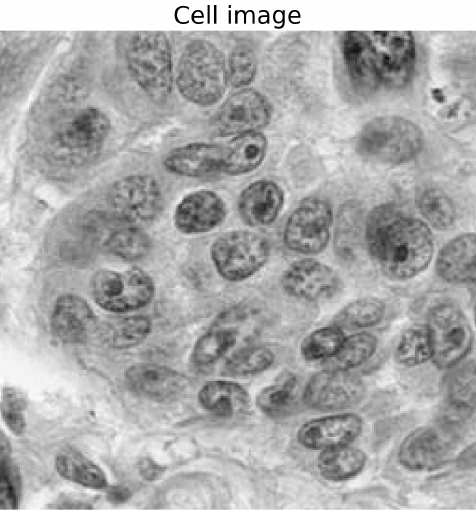
\includegraphics[width=\linewidth]{Materials/cell}
	\end{subfigure}
	\hfill
	\begin{subfigure}{0.32\linewidth}
		\centering
		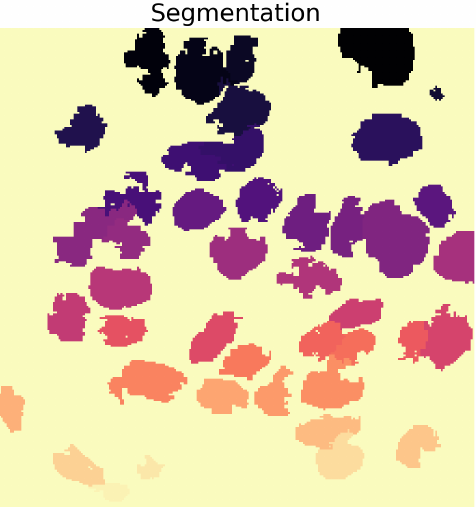
\includegraphics[width=\linewidth]{Materials/cellSeg}
	\end{subfigure}
	\hfill
	\begin{subfigure}{0.32\linewidth}
		\centering
		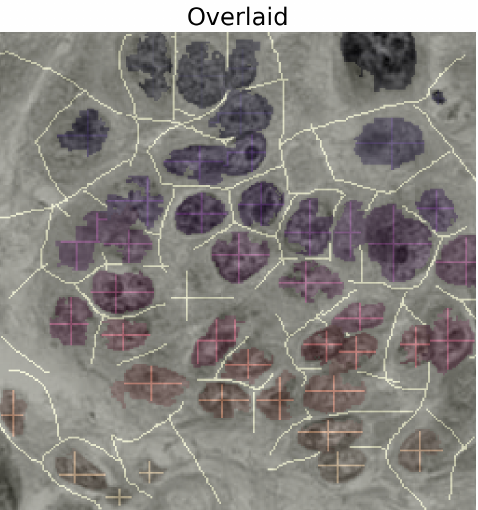
\includegraphics[width=\linewidth]{Materials/cellOverlaid}
	\end{subfigure}
	\caption{Original image, the final segmentation and markers, segmentation and original image overlaid.}
	\label{cellSeg}
\end{figure}

\begin{figure}
	\centering
	\begin{subfigure}{0.3\linewidth}
		\centering
		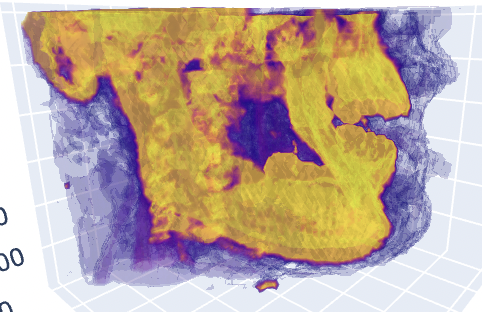
\includegraphics[width=\linewidth]{Materials/L3D}
		\caption{Right view on our data.}
	\end{subfigure}
	\hspace{1cm}
	\begin{subfigure}{0.3\linewidth}
		\centering
		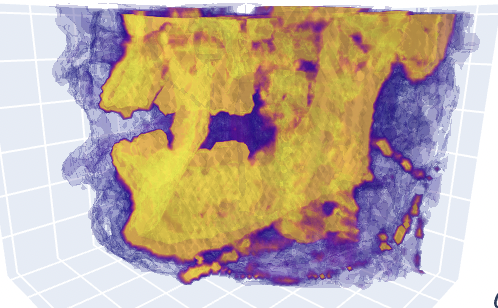
\includegraphics[width=\linewidth]{Materials/R3D}
		\caption{Left view on our data.\newline}
	\end{subfigure}
	\\
	\begin{subfigure}{0.3\linewidth}
		\centering
		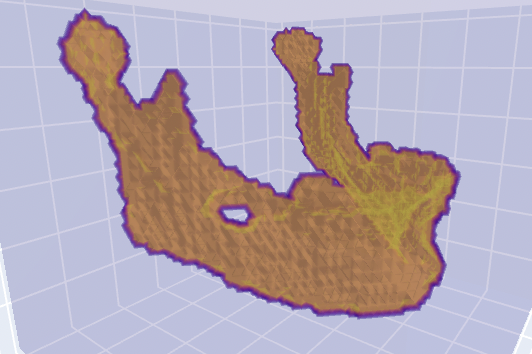
\includegraphics[width=\linewidth]{Materials/L3DSeg}
		\caption{Right view on segmentation.}
	\end{subfigure}
	\hfill
	\begin{subfigure}{0.3\linewidth}
		\centering
		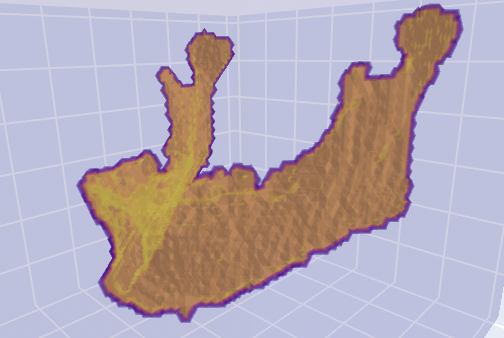
\includegraphics[width=\linewidth]{Materials/R3DSeg}
		\caption{Left view on Segmentation.}
	\end{subfigure}
	\hfill
	\begin{subfigure}{0.3\linewidth}
		\centering
		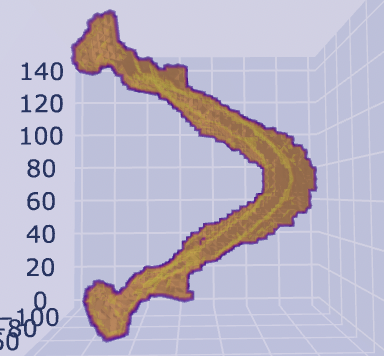
\includegraphics[width=\linewidth]{Materials/T3DSeg}
		\caption{Top view on segmentation.}
	\end{subfigure}
	\caption{Result of 3D segmentation of the mandible.}
	\label{mandible}
\end{figure}
Another algorithm which can be used for segmentation / to find object boundaries is Graph cut. Here the image is made to a graph representation and the more similar neighbouring pixels are, the more flow we allow between them. A max flow problem is then solved and a min cut is made to find the object boundary. As we are solving a max flow problem, this approach gives us an analytical solution to our segmentation problem opposed to the non-deterministic approach of using Random walker. This is a big advantage as the solution to the problem becomes consistent, however, it also requires it is possible to make a graph representation of the image and that it is possible to come up with a cost function. And even if this is possible, it requires that the graph representation can be contained in memory to be solved efficiently. Another issue could be boundaries are not 'clear' and a high amount of flow would go through what is supposed to be our boundaries, making it hard to make a min cut at an exact location. These issues are not present in the Random walker.\\
In conclusion, the Graph cut algorithm is preferred as it gives us an analytical solution, however it is not always possible to employ the Graph cut algorithm due to memory usage, cost function formulation or vague boundaries, but the Random walker algorithm solves these issues by being non-deterministic.